\documentclass[11pt,a4paper,openright,twoside]{book}
\def\myauthor{Adrià Arrufat}
\def\mytitle{Adaptive transforms for intra video coding}
\usepackage[british]{babel}
\usepackage{geometry}
\geometry{verbose,tmargin=2.5cm,bmargin=2.5cm,lmargin=2.5cm,rmargin=2.5cm}
\usepackage[nottoc]{tocbibind} % see http://www.howtotex.com/packages/how-to-add-bibliography-and-more-to-table-of-contents/
\usepackage{titlesec,titletoc} % to modify titles and add partial tocs
\usepackage[printonlyused,withpage]{acronym} % options: printonlyused, withpage
\usepackage{imakeidx} % allows customizing the index in the makeindex command
\usepackage{emptypage} % removes headers and footers from empty pages
\usepackage[thickqspace,amssymb,noams]{SIunits} % consistent units support
\usepackage{subfig}
\usepackage{nicefrac}
\usepackage{contour} % for inexisting bold symbols
\contourlength{0.01em}

% lines and paragraphs
% \usepackage{setspace}
% \setstretch{1}
% \parskip=\smallskipamount
% \setlength{\parindent}{0pt}

% font configuration
\usepackage{amsmath, amssymb}
% \usepackage{lmodern}
% \usepackage[default,scaled=0.85]{FiraSans}
% \usepackage[helvet]{sfmath}
% \usepackage[scaled=0.80]{sourcecodepro} % option: default
\usepackage[T1]{fontenc}
\usepackage{mathptmx}
\usepackage[scaled]{helvet}
% \usepackage{courier}

\usepackage[usenames,dvipsnames]{xcolor}
\usepackage{pgfplots,tikz}
\usepackage{bookmark} % needed for \bookmarksetup{startatroot}
\usepackage{hyperref}
\hypersetup{
	unicode=true,
	pdfencoding=auto,
	colorlinks=true,
	citecolor=blue,
	filecolor=red,
	linkcolor=Blue,
	urlcolor=blue,
	linktoc=all,
	pdfauthor={\myauthor},
	pdftitle={\mytitle},
	pdfsubject={video coding},
	pdfkeywords={video, image, transform},
	pdfinfo={
		CreationDate={D:20150121111947},
		%ModDate={...}
	},
}
% \urlstyle{same} % do not use monospaced fonts in urls

% Define a partial ToC to use at the beginning of every chapter
\providecommand{\chaptertoc}{
	\startcontents[chapters]
	\hrule
	\vspace{1em}
	\printcontents[chapters]{}{1}{{\bf\large Contents}}
	\hrule
}

\definecolor{almostwhite}{rgb}{0.9,0.9,0.95}
\providecommand{\todo}[1]{
	\begin{center}
		\colorbox{almostwhite}{
			\begin{minipage}{0.85\linewidth}
				\textbf{TODO:} #1
			\end{minipage}
		}
	\end{center}
}

\numberwithin{equation}{section} % equations referred to sections

\makeindex[options=-s index-alph-group.ist]

\title{\Huge\bf\mytitle}
\author{\myauthor}

\begin{document}
\frontmatter
\maketitle

\chapter*{Acknowledgements}
\label{cha:acknowledgements}
\addcontentsline{toc}{chapter}{Acknowledgements}

\setcounter{tocdepth}{5}
\tableofcontents
\addcontentsline{toc}{chapter}{Contents}
\cleardoublepage
\listoffigures
\cleardoublepage
\listoftables
\cleardoublepage

\mainmatter
\part{General introduction}
\label{prt:general_introduction}

\addcontentsline{toc}{section}{\protect\numberline{}Context}
\chapter*{Context}
\label{cha:context}

\part{State of the art}
\label{prt:state_of_the_art}

\chapter{Video coding fundamentals}
\label{sec:video_coding_fundamentals}
\chaptertoc

\section{Introduction to video coding}
\label{sec:introduction_to_video_coding}

\subsection{The need of video coding}
\label{sub:the_need_of_video_coding}

The purpose of video coding is to compress video files, which consist of
a sequence of images that, at some point, will be either transmitted or
stored.

For instance, a two-hour long film in \ac{HD} format ($1920 \times 1080$)
at a frame rate of 25 images per second and 8 bits to represent each one
of the \ac{RGB} channels, requires:
\[
	\frac{\unit{1920\times1080}{pix}}{\unit{1}{image}}
	\times \frac{\unit{25}{images}}{\unit{1}{s}}
	\times \unit{2}{\hour} \times \frac{\unit{3600}{s}}{\unit{1}{\hour}}
	\times \unit{3}{channels} \times \frac{\unit{8}{bits}}{\unit{1}{channel}}=
\]
\[
	= 8.957952 \times 10 ^ {12} \; \text{bits}
	= 8957.952\;\text{Gb} \approx 1043\;\text{GiB}
\]

Through this simple example, it is evident that video coding is
indispensable to store or stream video files.
Depending on the target quality, it is common to have compression rates
ranging from 100 to 1000.

For content providers, being able to reduce the size of the content they
broadcast implies increasing the number of contents they can store, as
well as the number of subscribers they can reach using the same
resources for storage and network capacity.

In 2013, two thirds of the \ac{IP} traffic was due to video
streaming, and this trend is only going to increase, reaching up to 84\%
of the \acs{IP} traffic by 2018~\cite{cisco-13-vni-forecast}.
Such statistics highlight the need of continuing the research on
new video coding techniques.

\section{The video coding system}
\label{sec:the_video_coding_system}

The video coding system describes a work flow to work with video
sequences.
It is composed of several stages, starting with the video acquisition at
the source and ending at the video display.
A good understanding of each part is crucial to be able to take the
proper decisions when delivering a video coding solution.

This section presents a scheme containing the most important concepts
used in state-of-the-art video coders.

Figure~\ref{fig:video_coding_system} describes how a complete video
coding system can be organised as a block diagram.

\begin{figure}[ht]
	\centering
	% \documentclass{book}
% \usepackage{tikz, libertine}
% \begin{document}
%
\pgfmathsetmacro{\nodebasesize}{1} % A node with a value of one will have this diameter
\pgfmathsetmacro{\nodeinnersep}{0.1}

\newcommand{\propnode}[5]{% position, name, options, value, label
	\pgfmathsetmacro{\minimalwidth}{sqrt (#4*\nodebasesize)}
	\node[#3,minimum width=\minimalwidth*1cm,inner sep=\nodeinnersep*0cm,circle,draw]
	(#2) at (#1) {#5};
}

\tikzstyle{bloq} = [rectangle, draw, text badly centered, minimum height=2.5em, inner sep=1mm]
\newcommand{\bloq}[4]{% position, name options, label
	\node[bloq,#3] (#2) at (#1) {\textsf{#4}};
}
\newcommand{\add}[2]{%position, name
	\draw (4,4) circle [radius=0.3] node (add) {\textsf$+$};
}

\begin{tikzpicture}[scale=1.5, x=1em, y=1em]
\tikzstyle{every node}=[font=\small]

	\def\startx{0}
	\def\starty{0}
	\def\thickness{thick}
	\def\hdist{5}
	\def\vdist{2}


	\bloq{\startx+0*\hdist,\starty-0*\vdist}{source}{text width=4.5em,fill=yellow!50}{\textsf{source}}
	\bloq{\startx+1*\hdist,\starty-0*\vdist}{pre}{text width=4.5em,fill=yellow!50}{\textsf{pre-processing}}
	\bloq{\startx+2*\hdist,\starty-0*\vdist}{encoding}{text width=4.5em,fill=yellow!50}{\textsf{encoding}}
	\bloq{\startx+3*\hdist,\starty-1*\vdist}{transmission}{text
	width=5.5em,fill=yellow!50}{\textsf{transmission}}
	\bloq{\startx+2*\hdist,\starty-2*\vdist}{decoding}{text width=4.5em,fill=yellow!50}{\textsf{decoding}}
	\bloq{\startx+1*\hdist,\starty-2*\vdist}{post}{text width=4.5em,fill=yellow!50}{\textsf{post-processing}}
	\bloq{\startx+0*\hdist,\starty-2*\vdist}{display}{text width=4.5em,fill=yellow!50}{\textsf{display}}

	\draw[-latex, \thickness] (source) -- (pre);
	\draw[-latex, \thickness] (pre) -- (encoding);
	\draw[-latex, \thickness] (encoding) -| (transmission);
	\draw[-latex, \thickness] (transmission) |- (decoding);
	\draw[-latex, \thickness] (decoding) -- (post);
	\draw[-latex, \thickness] (post) -- (display);

\end{tikzpicture}
% \end{document}

	\caption{Video coding system}
	\label{fig:video_coding_system}
\end{figure}

The composing blocks of the video system are explained more in detail in
the following subsections.

\subsection{Pre-processing}
\label{sub:pre_processing}

After the digital video has been acquired at the source, which may be of
many different sorts, such as natural scenes or synthetic
computer-generated content, it has to be processed in order to be
encoded.
Usually, the pre-processing stage can include some filtering, scaling
and colour space conversions on the raw video sequence.

\subsubsection{Colour space conversions}
\label{ssub:colour_space_conversions}
\index{HVS}
\index{YUV}
\index{gamma}
\index{luma}
\index{chroma}

Colour space conversions are used to change the colour
representation of the content to better fit the \ac{HVS}.
The raw video data is normally in \ac{RGB} format, corrected by the
transfer function of the camera ($\gamma$), hence denoted R'G'B'.

For historical reasons, in order to be backwards compatible with black
and white displays, the raw video file is converted to another colour
space that separates the light information (luma) from the colour
information (chroma), typically referred to as the YUV colour space
family~\cite{poynton-95-color-space}.
Moreover, due to the way the \ac{HVS} works, being more sensible to
light variations than to colour, this family of colour spaces supports
sub-sampling the chroma channels without any major perceptual
degradation.

\subsection{Encoding}
\label{sub:encoding}

This stage is in charge of converting the pre-processed raw video sequence
into a coded video stream to ease the storage and transmission.
A deep look at the inners of a widely used coding scheme is provided
in~\ref{sec:the_hybrid_video_coding_scheme}.

\subsection{Transmission}
\label{sub:transmission}

The transmission stage stands for the way the encoded bitstream is
transferred to the decoder.
Most typical examples are streaming and storage, which may determine
some of the encoder and decoder behaviours, like real time or memory
constraints.

\subsection{Decoding}
\label{sub:decoding}

As the stream is received by the decoder, it is buffered and used to
reconstruct the encoded data into the appropriate format, as signalled
by the encoder.
Video coding norms tend to define a standard video decoder, which
follows the implemented video coding specificication, such as \ac{AVC}
or \ac{HEVC}~\cite{itu-14-h265-hevc-rec,sullivan-12-overview-hevc}.
The encoder must comply to this specification by generating a decodable
stream.

\subsection{Post-processing}
\label{sub:post_processing}

The post-processing stage performs operations for image enhancement and
display adaptation, such as converting back to the original colour
space and to the display format.

\section{The hybrid video coding scheme}
\label{sec:the_hybrid_video_coding_scheme}

State-of-the-art video coding standards such as H.264/\acs{MPEG}-4 \acs{AVC}
and H.265/\acs{HEVC} use a hybrid video coding scheme that appeared in
H.261, in the late eighties.
Since then, all video coding standards and recommendations issued by the
\ac{ITU-T} and the \ac{MPEG} use it as their basic coding structure.

The hybrid video coding scheme is named after its use of both temporal
prediction and transform coding techniques for the prediction error.
A basic structure of the hybrid video coding scheme is presented in
figure~\ref{fig:hybrid_video_coding_scheme}.

\begin{figure}[ht]
	\centering
	% \documentclass{book}
% \usepackage{tikz, libertine}
% \begin{document}

\pgfmathsetmacro{\nodebasesize}{1} % A node with a value of one will have this diameter
\pgfmathsetmacro{\nodeinnersep}{0.1}

\newcommand{\propnode}[5]{% position, name, options, value, label
	\pgfmathsetmacro{\minimalwidth}{sqrt (#4*\nodebasesize)}
	\node[#3,minimum width=\minimalwidth*1cm,inner sep=\nodeinnersep*0cm,circle,draw] 
	(#2) at (#1) {#5};
}

\tikzstyle{bloq} = [rectangle, draw, text badly centered, minimum height=2.5em, inner sep=1mm]
\newcommand{\bloq}[4]{% position, name options, label
	\node[bloq,#3] (#2) at (#1) {\textsf{#4}}; 
}
\newcommand{\add}[2]{%position, name
	\draw (4,4) circle [radius=0.3] node (add) {\textsf$+$};
}


\begin{tikzpicture}[scale=1.5,x=1em,y=1em]
\tikzstyle{every node}=[font=\small]
	\def\x{0}
	\def\y{0}
	\def\thickness{thick}
	\def\h{2.0}
	\def\v{1.0}

\tikzstyle{frame} =
[rectangle, fill=white, draw, text badly centered, minimum width=3*\h em,minimum height=3*\v em]
% INPUT VIDEO SEQUENCE
	\draw (\x-\h,\y+0.5*\v) node[above] {\textsf{Input Video Sequence}};
	\draw (\x-\h,\y-3*\v) node[above] {\textsf{Split into blocks}};
	\node[frame] at (\x-\h-0.3,\y-\v+0.3){};
	\node[frame] at (\x-\h-0.2,\y-\v+0.2){};
	\node[frame] at (\x-\h-0.1,\y-\v+0.1){};
	\node[frame] (sequence) at (\x-\h,\y-\v){};
	\draw[step=0.25,thin,help lines] (\x,\y) grid (-2*\h,-2*\v);
	\draw[step=0.5,thin] (\x,\y) grid (-2*\h,-2*\v);
	\draw[step=1.0,black,thick] (\x,\y) grid (-2*\h,-2*\v);

	\filldraw[fill=blue!20, draw=blue!50,dashed,thick]
	(\x+1.5,\y-2.25*\v) --++ (7.5*\h,0) --++ (0,-15.25*\v) --++ (-7.5*\h,0) -- cycle;
	\node[above left] at (\x+4*\h,\y-6*\v) {\normalsize\textsf{Decoder}};

	\propnode{\x+1*\h,\y-1*\v}{add1}{fill=green!50}{0}{$+$}
	\propnode{\x+7*\h,\y-9*\v}{add2}{fill=green!50}{0}{$+$}
	\propnode{\x+0.75*\h/2,\y-1*\v}{inter1}{fill=black}{0.005}{}
	\propnode{2,\y-9*\v}{inter2}{fill=black}{0.005}{}
	\propnode{2,\y-14*\v}{inter3}{fill=black}{0.005}{}
	\propnode{3.5,\y-12*\v}{inter4}{}{0.005}{}
	\propnode{3.5,\y-16*\v}{inter5}{}{0.005}{}
	\propnode{8.5,\y-14*\v}{inter6}{fill=black}{0.005}{}
	\propnode{\x+5*\h,\y-10*\v}{inter7}{fill=black}{0.005}{}
	\propnode{\x+3*\h,\y-18.5*\v}{inter8}{fill=black}{0.005}{}

	\draw (\x+1.25*\h,\y-0.75*\v) node[above] {\textsf{residuals}};

	\bloq{\x+3*\h,\y-\v}{Transf}{text width=4.5em,fill=yellow!50}{Transform};
	\bloq{\x+5.5*\h,\y-\v}{Quant}{text width=4.5em,fill=yellow!50}{Quant.};
	\bloq{\x+7*\h,-\y-4*\v}{InvQuant}{text width=4.5em,fill=yellow!50}{Inv. Quant.};
	\bloq{\x+7*\h,\y-7*\v}{InvTransf}{text width=4.5em,fill=yellow!50}{Inv. Transform};
	\bloq{\x+3*\h,\y-12*\v}{IntraPred}{text width=4.5em,fill=yellow!50}{Intraframe\\Prediction};
	\bloq{\x+3*\h,\y-16*\v}{InterPred}{text width=4.5em,fill=yellow!50}{Interframe\\Prediction};
	\bloq{\x+3*\h,\y-20*\v}{MotionComp}{text width=4.5em,fill=yellow!50}{Motion\\Est./Comp.};
	\bloq{\x+10*\h,\y-10*\v}{EntrCod}{text width=4.5em,fill=yellow!50}{Entropy\\Coding};
	\bloq{\x+7*\h,\y-14*\v}{Reconst}{text width=6em,fill=white,minimum height=3em}{Reconst.\\images};

	\draw[-latex,\thickness] (sequence) -- (add1) node [below right] {\textsf{$-$}};
	\draw[-latex,\thickness] (add1) -- (Transf);
	\draw[-latex,\thickness] (Transf) -- (Quant);
	\draw[-latex,\thickness] (InvQuant) -- (InvTransf);
	\draw[-latex,\thickness] (InvTransf) -- (add2);
	\draw[-latex,\thickness] (add2) -- (Reconst);
	\draw[-latex,\thickness] (inter2) -- (add2);
	\draw[-latex,\thickness] (inter3) -- (add1);
	\draw[-latex,\thickness] (IntraPred) -- (inter4);
	\draw[-latex,\thickness] (InterPred) -- (inter5);
	\draw[-latex,\thickness] (inter3) -- (inter4);
	\draw[<->,help lines,\thickness] (inter3) ++(-45:\v) arc (-45:45:\v);
	\draw[dotted,help lines, \thickness] (inter3) -- (inter5);
	\draw[-latex,\thickness] (Reconst) --++ (2.5*\h,0) node [below,text width=3.5em,text badly centered] {\textsf{Output Video\\Signal}};
	\draw[-latex,\thickness] (EntrCod) --++ (0,-2*\v) node[below] {\textsf{bitstream}};
	\draw[-latex,\thickness] (Quant) -| (InvQuant);
	\draw[-latex,\thickness] (Quant) -| (EntrCod);
	\draw (\x+8.5*\h,\y-2.5*\v) node (TransCoeff) [right,text width=3em] {\textsf{Quant. Transf.\\Coeffs}};
	\draw[\thickness] (Reconst) -- (inter6);
	\draw[-latex,\thickness] (inter6) |- (IntraPred);
	\draw[-latex,\thickness] (inter6) |- (InterPred);
	% \draw[-latex,\thickness] (IntraPred) |- (EntrCod);
	\draw[-latex,\thickness] (inter1) |- (MotionComp);
	\draw[-latex, \thickness] (MotionComp) -- (InterPred);
	\draw[-latex, \thickness] (Reconst) |- (MotionComp);
	\draw[-latex, \thickness] (inter8) -| (inter7);
	\draw[-latex, \thickness] (IntraPred) |- (EntrCod);
	\draw (\x+8.1*\h,\y-9.5*\v) node [] {\textsf{Prediction data}};
\end{tikzpicture}
% \end{document}

	\caption{Hybrid video coding scheme}
	\label{fig:hybrid_video_coding_scheme}
\end{figure}

The hybrid video coding scheme provides an efficient way of compressing
a video signal into a bitstream of the smallest possible size.
The key features to achieve such a small bitstream are the signal
prediction and the transformation of the prediction error.

The encoder includes a decoder, represented inside a blue box, to be
able to perform its coding decisions based on what the decoder would do
while decoding a bitstream.

The building blocks of the hybrid video coding scheme are explained in
the following subsections.

\subsection{Partitioning}
\label{sub:partitioning}
\index{partitioning}

In order to process the video frames, they are exhaustively partitioned
into non-overlapping blocks.
These blocks ease the succeeding stages of prediction and transform.
The partitioning does not have to be uniform, allowing blocks of different
sizes to be used.
The optimal choice for the block size is left to the encoder.

\begin{figure}[ht]
	\centering
	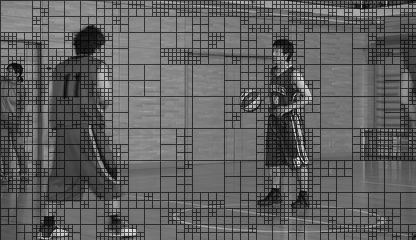
\includegraphics[width=0.6\linewidth]{./figures/partitioning-orig-all-001.png}
	\caption{Partitioning example using \acs{HEVC} at \acs{QP} 27}
	\label{fig:partitioning}
\end{figure}

\subsection{Prediction}
\label{sub:prediction}

Residual coding is video coding technique that, instead of coding the
blocks coming from the original source image directly, computes an
estimation of the block, which is then subtracted from the original
block, generating the residual block.
Those block estimations are carried out by the prediction module, using
some information from previously treated blocks.
This way, predictable information present in the original blocks will be
removed and their energy will be lowered.

Predictions must be performed the same way at both encoder and decoder
side, and this computed inside the blue box in
figure~\ref{fig:hybrid_video_coding_scheme}, referring to the decoder.
For this reason, the encoder uses reconstructed blocks (blocks that have
already been encoded and will make it to the bitstream) as the input
data to compute the predictions, because these blocks are equivalent to
those the decoder will handle.

Commonly, predictions might be of two types, depending on the origin of
the prediction source:
intra or spatial prediction for those blocks that
have been predicted using information within the same frame, and inter
or temporal prediction for those blocks predicted using other frames.

\begin{figure}[ht]
	\centering
	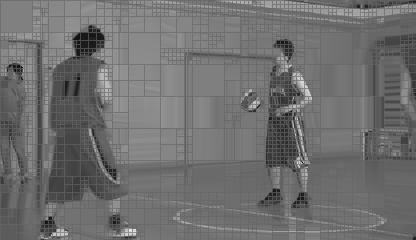
\includegraphics[width=0.6\linewidth]{./figures/partitioning-pred-all-001.png}
	\caption{Predicted image}
	\label{fig:predicted_image}
\end{figure}

\begin{figure}[ht]
	\centering
	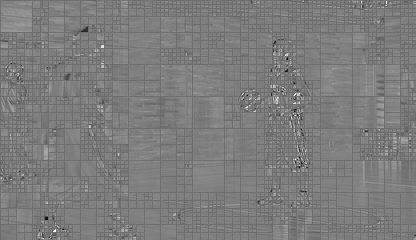
\includegraphics[width=0.6\linewidth]{./figures/partitioning-resi-all-001.png}
	\caption{Residual image (difference between original and predicted)}
	\label{fig:residual_image}
\end{figure}

\subsubsection{Intra prediction}
\label{ssub:intra_prediction}
\index{intra prediction}

Intra prediction, sometimes referred to as spatial prediction, is used
to remove correlation within local regions of a picture.
The basic principle of intra prediction is that the texture of a picture
region is similar to the texture of its neighbourhood and can be
predicted from there.

The intra prediction is analysed in
Chapter~\ref{cha:the_mode_dependent_directional_transforms}, when
introducing a kind of prediction-adapted transforms.

\subsubsection{Inter prediction}
\label{ssub:inter_prediction}
\index{inter prediction}

Inter prediction, or temporal prediction, takes advantage of the fact
that images close in time share many similarities, and that many of
their component regions will move as a whole.
Since the encoding order is not necessarily the same as the viewing
order, inter predictions can have their origins in either past or future
frames.
Regions that are covered and uncovered by other objects can be predicted
using this technique.

At the encoder side, an extra operation, called motion estimation, is
carried out.
This stage searches for the best matching area in the reference picture
for the current prediction block.
It is one of the most demanding parts of video coders, with regards to
the number of operations.

\subsection{Transform}
\label{sub:transform}

The transform stage removes remaining correlations from the residual
block, computed as the difference between the original and the predicted
blocks.
The goal of the transform is to concentrate the residual energy into as
many few coefficients as possible in the transform domain.

Considering that the subject of this thesis is centred around the
transforms for video coding, the transform stage will be explained
thoroughly in Chapter~\ref{cha:transform_coding}.

\subsection{Quantisation}
\label{sub:quantisation}
\index{QP}\index{lossy}\index{lossless}

The quantisation, applied in the transform domain, it is used to discard
any coefficient whose energy level is below a certain threshold.
High energy coefficients are also be affected by the quantisation.
In standards like \acs{HEVC}, the quantisation step is controlled by a
\ac{QP}.
It is worth noticing that it is the only non-reversible step in the whole
hybrid video coding scheme, and therefore what makes video coding lossy.
Lossless video coding can be attained by not using quantification in the
process.

% \begin{figure}[ht]
% 	\centering
% 	\subfloat[Partitioning]
% 	{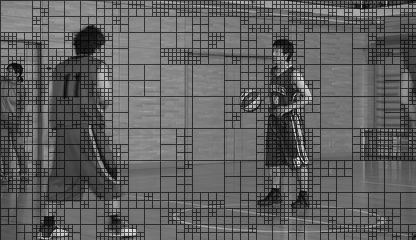
\includegraphics[width=0.8\linewidth]{./figures/partitioning-orig-all-001.png}}
% 	\\
% 	\subfloat[Predicted Image]
% 	{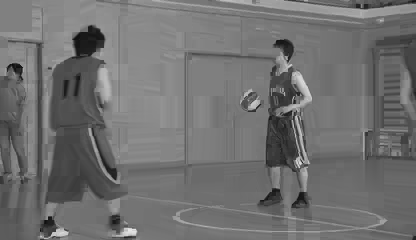
\includegraphics[width=0.8\linewidth]{./figures/pred_image-all-001.png}}
% 	\\
% 	\subfloat[Residual Image]
% 	{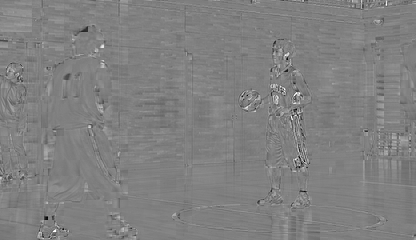
\includegraphics[width=0.8\linewidth]{./figures/res_image-all-001.png}}
% 	\caption{Example of an image at different encoding points for a
% 	certain level of quantisation}
% 	\label{fig:part_orig_pred_res_image}
% \end{figure}

\subsection{Entropy coding}
\label{sub:entropy_coding}
\index{CABAC}

Once the transform coefficients have been quantised, they have to be
treated to conform the bitstream.
That is, the transform coefficients are scanned to make sure they are
sorted in a way that will make the entropy coder work more efficiently.
Signalling is also conveyed into the bitstream at this point, and the
entropy coder ensures a correct binarisation while using the adequate
number of bits thanks to the \ac{CABAC}.

\section{Encoder control}
\label{sec:encoder_control}

The encoder control is used by essentially all blocks in the diagram
from figure~\ref{fig:hybrid_video_coding_scheme}.
This technique allows the encoder to take decisions related to coding
based on the application requirements.
These decisions include the block sizes and the prediction to use.
For each block size and kind of prediction, the encoder computes the
distortion, using its own decoder, and estimates the rate as illustrated
in figure~\ref{fig:rate_distortion_scheme}.

\begin{figure}[ht]
	\centering
	% \documentclass{book}
% \usepackage{tikz}
% \usepackage{mathptmx}
% \usepackage[scaled=0.92]{helvet}
% \begin{document}

\pgfmathsetmacro{\nodebasesize}{1} % A node with a value of one will have this diameter
\pgfmathsetmacro{\nodeinnersep}{0.1}

\newcommand{\propnode}[5]{% position, name, options, value, label
	\pgfmathsetmacro{\minimalwidth}{sqrt (#4*\nodebasesize)}
	\node[#3,minimum width=\minimalwidth*1cm,inner sep=\nodeinnersep*0cm,circle,draw] 
	(#2) at (#1) {#5};
}

\tikzstyle{bloq} = [rectangle, draw, text badly centered, minimum height=2.5em, inner sep=1mm]
\newcommand{\bloq}[4]{% position, name options, label
	\node[bloq,#3] (#2) at (#1) {\textsf{#4}}; 
}
\newcommand{\add}[2]{%position, name
	\draw (4,4) circle [radius=0.3] node (add) {\textsf$+$};
}

\begin{tikzpicture}[scale=1.5, x=1em, y=1em]
\tikzstyle{every node}=[font=\small]

	\def\startx{0}
	\def\starty{0}
	\def\thickness{thick}
	\def\hdist{5}
	\def\vdist{3}

	\filldraw[fill=blue!20, draw=blue!50,dashed,thick]
	(\startx-2.5,\starty+2) --++ (15,0) --++ (0,-4) --++ (-15,0) -- cycle;
	\filldraw[fill=blue!20, draw=blue!50,dashed,thick]
	(\startx-2.5,\starty-\vdist-1) --++ (15,0) --++ (0,-4) --++ (-15,0) -- cycle;

	\bloq{\startx+0*\hdist,\starty-0*\vdist}{transf}{text width=5.0em,fill=yellow!50}{\textsf{transform}}
	\bloq{\startx+1*\hdist,\starty-0*\vdist}{quant}{text width=5.0em,fill=yellow!50}{\textsf{quantisation}}
	\bloq{\startx+2*\hdist,\starty-0*\vdist}{entrocod}{text width=5.0em,fill=yellow!50}{\textsf{entropy coding}}

	\bloq{\startx+2*\hdist,\starty-2*\vdist}{entrodec}{text width=5.0em,fill=yellow!50}{\textsf{entropy decoding}}
	\bloq{\startx+1*\hdist,\starty-2*\vdist}{iquant}{text width=5.0em,fill=yellow!50}{\textsf{inverse quantisation}}
	\bloq{\startx+0*\hdist,\starty-2*\vdist}{itransf}{text width=5.0em,fill=yellow!50}{\textsf{inverse transform}}

	\node (rate) at (\startx+3*\hdist,\starty-1*\vdist) {\textsf{rate}};
	\node [label={[xshift=0cm, yshift=0.5cm]\textsf{encoder}}] at (quant) {};
	\node [label={[xshift=0cm, yshift=-1.2cm]\textsf{decoder}}] at (iquant) {};

	\draw[latex-, \thickness] (transf) -- (-4,0) node [left] (in) {\large$x$};
	\draw[-latex, \thickness] (itransf) -- (-4,-2*\vdist) node [left] (out) {\large$\hat x$};

	\node (dist) at (-4.425,-\vdist) {\textsf{distortion}};

	\draw [-latex, \thickness] (dist) -- (in);
	\draw [-latex, \thickness] (dist) -- (out);

	\draw[-latex, \thickness] (transf) -- (quant);
	\draw[-latex, \thickness] (quant) -- (entrocod);
	\draw[\thickness] (entrocod) -| (rate);
	\draw[-latex, \thickness] (rate) |- (entrodec);
	\draw[-latex, \thickness] (entrodec) -- (iquant);
	\draw[-latex, \thickness] (iquant) -- (itransf);


\end{tikzpicture}
% \end{document}

	\caption{Rate-distortion scheme of a transform-based codec}
	\label{fig:rate_distortion_scheme}
\end{figure}

\subsection{Distortion measures}
\label{sub:distortion_measures}

\subsubsection{Mean squared error}
\label{ssub:mean_squared_error}
\index{MSE}

The \ac{MSE} is the average of the square difference between two
signals.
For two-dimensional signals, such as images, the \ac{MSE} can be computed as:

\begin{equation}
	MSE_{I,K} = \frac{1}{m\,n} \sum\limits_{i=0}^{m-1} \sum\limits_{j=0}^{n-1}
	{\left[ I(i,j) - K(i,j) \right]} ^2
	\label{eqn:mse}
\end{equation}

Where $I$ and $K$ are two images of $m \times n$ pixels.

\subsubsection{Peak signal-to-noise ratio}
\label{ssub:peak_signal_to_noise_ratio}
\index{PSNR}

The \ac{PSNR} is an objective quality measure that computes the ratio
between the maximum possible value of a signal and the power of the
noise that affects the fidelity of its approximation.
It is usually defined in terms of the logarithmic decibel scale to cope
with the wide range that signals might have.
Defining the \ac{PSNR} in terms of the \ac{MSE} from
equation~\ref{eqn:mse}, it can be expressed as:
\begin{equation}
	PSNR = 10 \log_{10} \left(\frac{MAX_I^2}{MSE_{I,K}}\right)
	= 20 \log_{10} (MAX_I) - 10 \log_{10} (MSE_{I,K})
	\label{eqn:psnr}
\end{equation}
For 8-bit depth images, $MAX = 2^{8} - 1 = 255$.

\subsection{Rate-distortion optimisation}
\label{sub:rate_distortion_optimisation}
\index{RDO}

In order to carry out the most sensible decision at each time, the
encoder uses a \ac{RDO} criterion
\cite{sullivan-98-rdo-video-compression}.

Each time the encoder has to make a decision about choosing a
particular block size for the partitioning or a prediction mode, it
checks the distortion that decision might cause as well as an estimation
of the bit rate needed.
The encoder performs this computation iteratively the same block,
exploring many different coding possibilities and finally selects the
one that provides the best score in terms of rate and distortion.
This is called the \ac{RDO} loop.

As seen in the previous subsections, computing the distortion is
reasonably straightforward.
However, estimating the bit rate is a bit more delicate, since the whole
entropy coder cannot be run each time the encoder explores the different
possibilities for a block.
As a consequence, an estimation of the bit rate is used in the \ac{RDO}
loop.

\section{Bj{\o}ntegaard Delta measurements}
\label{sub:bjontegaard_delta_measurements}
\index{BD-rate}
\index{BD-PSNR}

Comparing two video coding techniques objectively might be complicated,
as both distortion and bit rate savings have to be taken into account.

Metrics introduced by Gisle Bj{\o}ntegaard, know as \ac{BD} measurements
have become the current \emph{de facto} standard to objectively compare
the result of two encodings~\cite{VCEG-M33,VCEG-AI11}.
Two different metrics are defined:
\begin{itemize}
	\item \ac{BD}-rate: computes the relative savings in bit rate for an
		equivalent distortion in percent.
	\item \ac{BD}-\ac{PSNR}: computes the relative quality improvement
		in \deci\bel.
\end{itemize}

% TODO
\todo{
\begin{itemize}
	\item Maybe place this section elsewhere.
	\item Graphical examples as in Wien's book~\cite{wien-15-hevc}.
\end{itemize}
}

\section{Conclusions}
\label{sec:conclusions_video_coding}

This chapter has presented the motivation for video coding as well as
some general concepts concerning an overview of the video coding system.

Current video coders exploit both redundancies existing within images of
the video sequence via predictions.
These predictions can be either spatial or temporal, depending on
whether the prediction source is the same image or another image,
respectively.
Unpredictable parts of the image, called residuals, are then transformed
in order to concentrate their energy in as few coefficients as possible.

Next chapter will explore the details of the transforms used in video
coding, namely their design principles and a comparison between two
design approaches.

\chapter{Transform coding}
\label{cha:transform_coding}
\chaptertoc

\section{Introduction to transforms}
\label{sec:introduction_to_transforms}

In the previous chapter, transforms were mentioned as an important part
in current video coders.
This chapter will study their design and properties that lead transforms
to be useful in video coding.

A transform is a mathematical operation that takes an input signal and
represents the same input signal in a different domain.

High energy compaction provided by transform coding has led this
technique to be present in the international video coding standards.

Transform coding allows removing existing signal correlations in the
spatial domain, leading to a decorrelated signal in the transform
domain.
This is of great importance for the upcoming stages of scanning and
entropy coding.

Transforms can be very abstract since they tend to work in N-dimensional
spaces.
However, restraining ourselves to two dimensions, one of the most visual
and representative example of transforms are rotations.
The example in figure~\ref{fig:transform_rotation} helps visualising the
transform role in signal compression.

\begin{figure}[ht]
	\centering
	% \documentclass{book}
% \usepackage{tikz, libertine, ifthen}
% \begin{document}
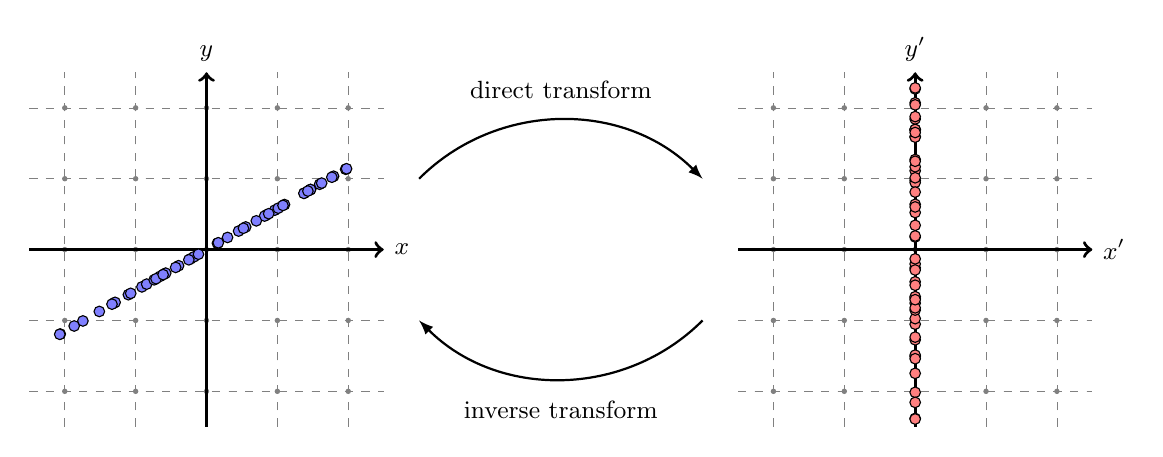
\begin{tikzpicture}[scale=0.9]
\tikzstyle{every node}=[font=\small]

	\draw[style=help lines, dashed, very thin, rotate=0] (0.5,0.5) grid (5.5,5.5);
	\draw[style=help lines, dashed, very thin, rotate=0] (10.5,0.5) grid (15.5,5.5);

	\foreach \x in {1,2,...,5} {
		\foreach \y in {1,2,...,5} {
			\filldraw [black!50, opacity = 1] (\x,\y) circle (0.03);
		}
	}

	\foreach \x in {11,12,...,15} {
		\foreach \y in {1,2,...,5} {
			\filldraw [black!50, opacity = 1] (\x,\y) circle (0.03);
		}
	}

	\def\seed{88}
	\pgfmathsetmacro{\xvar}{2.4}
	\pgfmathsetmacro{\yvar}{0.0}

	\def\angle{30}
	\pgfmathsetseed{\seed}
	\pgfmathsetmacro{\xoff}{3}
	\pgfmathsetmacro{\yoff}{3}
	\draw[style=help lines, dashed, very thin, rotate=0]
		(\xoff-2.5,\yoff-2.5) grid (\xoff+2.5,\yoff+2.5);
	\draw[->,very thick] (\xoff-2.5,\yoff)--(\xoff+2.5,\yoff) node[right]{$x$};
	\draw[->,very thick] (\xoff,\yoff-2.5)--(\xoff,\yoff+2.5) node[above]{$y$};
	\pgfmathsetmacro{\radius}{0.075}
	\foreach \i in {1,2,...,50} {
		\pgfmathsetmacro{\x}{(rand) * \xvar}
		\pgfmathsetmacro{\y}{(rand) * \yvar}
		\pgfmathsetmacro{\xrot}{\x*cos(\angle) - \y*sin(\angle) + \xoff}
		\pgfmathsetmacro{\yrot}{\x*sin(\angle) + \y*cos(\angle) + \yoff}
		\filldraw [black, fill=blue!50] (\xrot,\yrot) circle (\radius);
	}

	\def\angle{90}
	\pgfmathsetseed{\seed}
	\pgfmathsetmacro{\xoff}{13}
	\pgfmathsetmacro{\yoff}{3}
	\draw[style=help lines, dashed, very thin, rotate=0]
		(\xoff-2.5,\yoff-2.5) grid (\xoff+2.5,\yoff+2.5);
	\draw[->,very thick] (\xoff-2.5,\yoff)--(\xoff+2.5,\yoff) node[right]{$x'$};
	\draw[->,very thick] (\xoff,\yoff-2.5)--(\xoff,\yoff+2.5) node[above]{$y'$};
	\foreach \i in {1,2,...,50} {
		\pgfmathsetmacro{\x}{(rand) * \xvar}
		\pgfmathsetmacro{\y}{(rand) * \yvar}
		\pgfmathsetmacro{\xrot}{\x*cos(\angle) - \y*sin(\angle) + \xoff}
		\pgfmathsetmacro{\yrot}{\x*sin(\angle) + \y*cos(\angle) + \yoff}
		\filldraw [black, fill=red!50] (\xrot,\yrot) circle (\radius);
	}

	\draw [thick,-latex] (6,4) to [in=135,out=45] ++ (4,0);
	\draw [thick,latex-] (6,2) to [in=-135,out=-45] ++ (4,0);
	\node [above] at (8,5) {direct transform};
	\node [below] at (8,1) {inverse transform};
\end{tikzpicture}
% \end{document}

	\caption{Simple transform performing a rotation}
	\label{fig:transform_rotation}
\end{figure}

Whereas on the left signal (in blue), both the horizontal and vertical
dimensions are needed to describe the signal completely, on the right
signal (in red), the vertical dimension is enough to provide an equally
accurate signal representation, since the horizontal dimension remains
constant.

\subsection{Block-based transforms}
\label{sub:block_based_transforms}

Amongst all the different kinds of transforms available, the ones used
in image and video coding applications are the block-based transforms
due to the good trade-off they provide in terms of complexity and
performance.

\subsection{Separability}
\label{sub:separability}

Image and video coding deal with image blocks, which are two-dimensional
signals and, consequently, use transforms able two deal with those
signals.

The naive approach to work with those signals is to use non-separable
transforms.
These transforms take the signal as a whole and reshape it to a
single-dimensional signal.
Afterwards the transform is applied normally.
The main disadvantage of this approach is the number of calculations
required to obtain the transformed signal.

\subsection{Transform design}
\label{sub:transform_design}

\def\A{\mathbf{A}}
\def\I{\mathbf{I}}
\def\P{\text{P}}
\def\U{\mathbf{U}}
\def\V{\mathbf{V}}
\def\X{\mathbf{X}}
\def\Y{\mathbf{Y}}
\def\arg{\text{arg}}
\def\c{\mathbf{c}}
\def\d{\text{d}}
\def\e{\text{e}}
\def\GGD{\text{GGD}}
\def\tr{\text{tr}}
\def\x{\mathbf{x}}
\def\Lambdab{\contour[3]{black}{$\Lambda$}}

\begin{equation}
	J(\lambda) = \text{Distortion} + \lambda \text{Rate}
\end{equation}

\begin{equation}
	J(\lambda) = \sum\limits_{\forall i}{\Vert \x_i - \A^T \c_i \Vert}_2^2
	+ \lambda r_i
\end{equation}

Next sections will study different transform design approaches, based on
different modellings of the rate constraint.

\section{The Karhunen-Loève transform}
\label{sec:the_karhunen_loeve_transform}
\index{KLT}
The \ac{KLT}~\cite{rao-01-transform-data-compression-book}

\section{The rate-distortion optimised transforms}
\label{sec:the_rate_distortion_optimised_transforms}
\index{RDOT}

In order to better fit the video coding demands, Sezer proposes a kind
of transforms that take into account the sparsity of the output in their
design~\cite{sezer-11-phd}.
The proposed \ac{RDOT} can be expressed as:
\begin{equation}
	\A_{opt} = \arg\min\limits_{\A}
	\sum_{\forall i} \min\limits_{\c_i}
	\left(
	{\Vert \x_i - \A^T\c_i \Vert}_2^2 + \lambda\overline{\Vert \c_i \Vert}_0
	\right)
	\label{eqn:rdot-nsep}
\end{equation}
Where $\x_i$ are the input signals, i.e.\ a block of the training set,
$\c_i$ are its quantised transformed coefficients using the transform
$\A$.
$\A^T$ is its transposed matrix, as $\A$ is chosen orthonormal.
The constraint in the cost function is the average $\ell_0$ norm of the
coefficients, i.e.\ the number of non-zero coefficients.
Finally, $\lambda$ is the Lagrange multiplier of the constraint.

A thorough study of equation~\ref{eqn:rdot-nsep} analysing its
properties and consequences is detailed below.

\subsection{The \acs{RDOT} metric}
\label{sub:the_rdot_metric}

The value that \acp{RDOT} minimise is expressed in
equation~\ref{eqn:rdot_metric} for a single signal.
As it is explicitly written, this metric depends exclusively on the
quantisation step $\Delta$ and the initial transform used $\A$.
\begin{equation}
	\delta_{\Delta,\A} (\lambda) =
	{\Vert \x - \A^T \c \Vert}_2^2 + \lambda\overline{\Vert \c \Vert}_0
	\label{eqn:rdot_metric}
\end{equation}
The first part of the equation represents the distortion introduced by
the quantisation.
The second term serves as rate-like constraint, by ensuring that the
number of significant values in the transform domain is minimised,
together with the distortion.

The minimisation of the metric happens in two steps, iteratively until
convergence:
\begin{enumerate}
	\item Finding the optimal coefficients for a given transform.
	\item Updating the transform for the optimal coefficients.
\end{enumerate}

\subsubsection{Optimal coefficients for a given transform}
\label{ssub:optimal_coefficients_for_a_given_transform}

The optimal coefficients are obtained by transforming the signal and
hard-thresholing them:
\begin{equation}
	\c = \lfloor \X \rfloor = \lfloor \A \x \rfloor
\end{equation}
The threshold value is tightly related to the Lagrange multiplier $\lambda$,
as demonstrated in Section~\ref{sub:the_lagrange_multiplier}:
\begin{equation}
	\c[n] =
	\begin{cases}
		\X[n] & \vert \X[n] \vert \ge \displaystyle \frac{\Delta}{2} \\
		0     & \text{otherwise} \\
	\end{cases}
	\label{eqn:hard_threshold}
\end{equation}

\subsubsection{Optimal transform for given coefficients}
\label{ssub:optimal_transform_for_given_coefficients}

Once the optimal coefficients have been found, the transform $\A$ must
be updated to provide the mapping between $\x$ and $\c$ while minimising
the reconstruction error.
\begin{equation}
	\A_{opt} = \arg\min\limits_{\A}
	\left(
	\sum_{\forall i}{\Vert \x_i - \A^T\c_i\Vert}^2
	\right)
	\qquad \text{s.t. } \A\A^T = \I
\end{equation}
Since the expression represents a scalar value, it can be rewritten
using the trace:
\begin{equation}
	\A_{opt} = \arg\min\limits_{\A}
	\left(\sum_{\forall i}\tr\left( 
	{\left(\x_i - \A^T\c_i\right)}^T\left( \x_i - \A^T\c_i\right)
	\right)\right)
\end{equation}
Operating:
\begin{equation}
	\A_{opt} = \arg\min\limits_{\A}
	\left(\sum_{\forall i}\tr\left( 
	\x_i^T\x_i -\x_i^T\A^T\c_i -\c_i^T\A\x_i^T + \c_i^T\A\A^T\c_i
	\right)\right)
\end{equation}
Since the trace is a linear operator and $\A\A^T=\I$:
\begin{equation}
	\A_{opt} = \arg\min\limits_{\A}
	\left(\sum_{\forall i}
	\tr\left(\x_i^T\x_i\right)
	-\tr\left(\x_i^T\A^T\c_i\right)
	-\tr\left(\c_i^T\A\x_i^T\right)
	+\tr\left(\c_i^T\c_i \right)
	\right)
\end{equation}
Making use of the cyclic property of the trace and removing
$\A$-independent terms:
\begin{equation}
	\A_{opt} = \arg\min\limits_{\A}
	\left(\sum_{\forall i}
	-2\tr\left(\c_i\x_i^T\A^T\right)
	\right)
\end{equation}
We now define $\Y=\displaystyle\sum_{\forall i}\c_i\x_i^T$ and its SVD
decomposition $\Y=\U\Lambdab^{\nicefrac{1}{2}}\V^T$, where $\U$ and $\V$
are orthonormal and $\Lambdab$ is diagonal.
The equation rewrites as follows:
\begin{equation}
	\A_{opt} = \arg\min\limits_{\A}
	\left(
	-2\tr\left(\U\Lambdab^{\nicefrac{1}{2}}\V^T\A^T\right)
	\right)
\end{equation}
Minimising a negative expression is equivalent to maximise its positive
version.
Re-arranging the terms using the trace cyclic property:
\begin{equation}
	\A_{opt} = \arg\min\limits_{\A}
	\left(
	-2\tr\left(\Lambdab^{\nicefrac{1}{2}}\V^T\A^T\U\right)
	\right)
\end{equation}
Let $\P=\V^T\A^T\U$. Since $\V$, $\A$ and $\U$ are orthonormal, so is
$\P$. The equation is now:
\begin{equation}
	\A_{opt} = \arg\max\limits_{\A}
	\left(
	\tr\left(\Lambdab^{\nicefrac{1}{2}}\P\right)
	\right)
\end{equation}
Since $\Lambdab$ is a diagonal matrix whose entries are non-negative by
definition and $\P$ is orthonormal, the maximisation is achieved when
$\P=\I$
\begin{equation}
	\V^T\A_{opt}^T\U=\I\quad \Rightarrow \quad \A_{opt} = \U\V^T
\end{equation}

\subsection{The Lagrange multiplier}
\label{sub:the_lagrange_multiplier}

It is a well-known fact that the residuals distribution can be modelled
quite accurately using a generalised normal distribution or \ac{GGD}.

\index{generalised normal distribution}
\index{generalised gaussian distribution}
\index{exponential power distribution}
Figure~\ref{fig:probability_density_functions} illustrates the \acp{PDF}
of a set of residuals transformed with the \ac{DCT} and the same residuals
transformed with an adapted \ac{RDOT}.
Since residuals are the difference between the predicted block and the
original block, errors in prediction are made by excess or defect
evenly, so their mean is zero.
As expected, the use of an adapted transformed has increased the number
of zeroes in the transform domain and, consequently, lowered the amount
of values elsewhere.
When changing the transform, the resulting \ac{PDF} is changed, but
since the transforms are orthonormal, the variance remains the same.
\begin{figure}[ht]
	\centering
	\vspace{0.30\textheight} % using this to speedup compilation
	% \definecolor{mygreen}{RGB}{0,143,0}
\begin{tikzpicture}[
	declare function={gamma(\z)=
    (2.506628274631*sqrt(1/\z) + 0.20888568*(1/\z)^(1.5) + 0.00870357*(1/\z)^(2.5) - (174.2106599*(1/\z)^(3.5))/25920 - (715.6423511*(1/\z)^(4.5))/1244160)*exp((-ln(1/\z)-1)*\z);},
	declare function={b(\s,\g)=
	1/\s*sqrt(gamma(3/\g)/gamma(1/\g));},
	declare function={a(\s,\g)=
	b(\s,\g)*\g/(2*gamma(1/\g));},
	declare function={ggd(\s,\g,\x)=
	a(\s,\g)*exp(-(abs(\x)*b(\s,\g))^\g);}
]
	\pgfplotsset{/tikz/font={\small}}
	\begin{axis}[
			xlabel={Values},
			ylabel={Density},
			grid=both,
			scale only axis,
			width=0.80\textwidth,
			height=0.30\textheight,
			scaled y ticks = false,
			% xtick={0,2,...,22},
			% x tick label style={
			% 	/pgf/number format/.cd,
			% 	set thousands separator={\thinspace},
			% 	/tikz/.cd
			% },
			% ytick={0,0.01,...,0.09},
			y tick label style={
				/pgf/number format/.cd,
				set decimal separator={.},
				fixed,
				fixed zerofill,
				precision=2,
				/tikz/.cd
			},
			xmin=-20, xmax=20,
			ymin=0, ymax=0.14,
			legend style={nodes=right},
			legend pos= north east,
			unbounded coords=jump,
		]

		\pgfplotstableread{figures/pdf_dct.dat}\table
		\addplot[black, thick, smooth, tension=0.3]
		table[x=x,y=dct,col sep=tab] from \table;
		\addlegendentry{DCT}

		\pgfplotstableread{figures/pdf_rdot.dat}\table
		\addplot[red, thick, smooth, tension=0.3]
		table[x=x,y=rdot,col sep=tab] from \table;
		\addlegendentry{RDOT}

		\addplot[blue, dotted, thick, samples=51, smooth, domain=-20:20]
		{ggd(5.1,1,x)};
		\addlegendentry{GGD($\sigma$,1,$x$)}

		\addplot[mygreen, dashed, thick, samples=51, smooth, domain=-20:20]
		{ggd(5.1,2,x)};
		\addlegendentry{GGD($\sigma$,2,$x$)}
	\end{axis}
\end{tikzpicture}

% vim:set filetype=tex:

	\caption{\acsp{PDF} of the residuals with different transforms
	compared to Laplace and normal distributions}
	\label{fig:probability_density_functions}
\end{figure}
Figure~\ref{fig:probability_density_functions} also includes the
\ac{PDF} of a Laplace distribution and a normal distribution.
Those two distribution are particular cases of a \ac{GGD}.

For this reason, in order to obtain the optimal Lagrange multiplier in a
reasonably general case, a \ac{GGD} will be used to represent the
residuals \ac{PDF}.
The centred \ac{GGD} \ac{PDF} can be expressed compactly as:
\index{gamma function}
\begin{equation}
	\GGD(\sigma,\gamma,x)=
	a\e^{-{\left(b\vert x \vert\right)}^\gamma}
	\label{eqn:ggd}
\end{equation}
Where:
\begin{align}
	b &= \frac{1}{\sigma}\sqrt{
	\frac{\Gamma\left(\nicefrac{3}{\gamma}\right)}
	{\Gamma \left(\nicefrac{1}{\gamma}\right)}} \\
	a &= \frac{b\gamma}{2\Gamma \left(\nicefrac{1}{\gamma}\right)}
\end{align}
and $\Gamma(z)$ is the gamma function, defined as:
\begin{equation}
	\Gamma(z) = \int_0^\infty t^{z-1}\e^{-t}\d t
\end{equation}
\index{Laplace distribution}
\index{gaussian distribution}
\index{normal distribution}
\index{uniform distribution}
The Laplace and normal or Gaussian \acp{PDF} are achieved with
$\gamma=1$ and $\gamma=2$, respectively.
Even the uniform distribution can be reached by making $\gamma\to\infty$.
However, from figure~\ref{fig:probability_density_functions} one can see
that $1\le\gamma\le2$ for video residuals.

In order to find the optimal $\lambda$, equation~\ref{eqn:rdot_metric}
has to be derived.
The problem will be tackled in two separated steps:
\begin{enumerate}
	\item Compute the distortion analytically and derive it.
	\item Compute the rate constraint and derive it.
\end{enumerate}

\subsubsection{Derivation of the distortion function}
\label{ssub:derivation_of_the_distortion_function}

The distortion introduced by the hard-thresholding from
equation~\ref{eqn:hard_threshold} can be expressed as:
\begin{equation}
	D
	= \int_{-\infty}^{\infty} {(x - \hat x)}^2 \P_X (x)\d x
	= \int_{-\infty}^{\infty} \left(x^2 -2x\hat x + {\hat x}^2\right) \P_X (x)\d x
	= \int_{\nicefrac{-\Delta}{2}}^{\nicefrac{\Delta}{2}}
	x^2\P_X (x) \d x
\end{equation}
Note that the integration intervals have been reduced to where the
quantised values differ from the original ones, that is, the values that
have been affected by the hard-thresholding from
equation~\ref{eqn:hard_threshold}.

Substituting $P_X(x)$ by the residuals \ac{PDF}:
\begin{align}
	D
	&=\int_{\nicefrac{-\Delta}{2}}^{\nicefrac{\Delta}{2}}
	x^2 a \e^{-{\left(b\vert x \vert\right)}^\gamma} \\
	&=2 \int_0^{\nicefrac{\Delta}{2}}
	x^2 a \e^{-{\left(b x \right)}^\gamma} \\
	&=
		2a \frac{\Gamma\left(\frac{3}{\gamma}\right)-
		\Gamma\left(
		\frac{3}{\gamma},{\left(\frac{b\Delta}{2}\right)}^\gamma
		\right)}{b^3\gamma}
	\label{eqn:distortion}
\end{align}
Where $\Gamma(a,z)$ is the incomplete upper gamma function, defined as:
\index{incomplete upper gamma function}
\begin{equation}
	\Gamma(a,z)=\int_z^\infty t^{a-1}\e^{-t}\d t
\end{equation}
Deriving equation~\ref{eqn:distortion} in $\Delta$:
\begin{equation}
	\frac{\partial D}{\partial\Delta} =
	\frac{\Delta^2 a \e^{{(-b\nicefrac{\Delta}{2})}^\gamma}}{4}
	\label{eqn:diff_distortion}
\end{equation}

\subsubsection{Derivation of the zero norm function}
\label{ssub:derivation_of_the_zero_norm_function}

By definition, the $\ell_0$ norm is the total number of non-zero
elements in a vector.
Consequently, the constraint can be expressed as:
\begin{equation}
	R 
	= \overline{\Vert \c \Vert}_0 = \frac{1}{N}{\Vert \c \Vert}_0
	= \frac{1}{N} N \P_X\left(\vert X \vert \ge \frac{\Delta}{2}\right)
	= 1-P_X\left(\vert X \vert < \frac{\Delta}{2}\right)
	= 1-\int_{\nicefrac{-\Delta}{2}}^{\nicefrac{\Delta}{2}}\P_X(x)\d x
\end{equation}
Substituting $P_X(x)$ by the residuals \ac{PDF}:
\begin{align}
	R
	&=1-\int_{\nicefrac{-\Delta}{2}}^{\nicefrac{\Delta}{2}}
	a \e^{-{\left(b\vert x \vert\right)}^\gamma} \\
	&=1-2\int_0^{\nicefrac{\Delta}{2}}
	a \e^{-{\left(b x \right)}^\gamma} \\
	&=1+2a\frac{\Gamma\left(
		\frac{1}{\gamma},{\left(\frac{b\Delta}{2}\right)}^\gamma\right)-
		\Gamma\left(\frac{1}{\gamma}\right)}
		{b\gamma}
	\label{eqn:rate}
\end{align}
Deriving equation~\ref{eqn:rate} in $\Delta$:
\begin{equation}
	\frac{\partial R}{\partial\Delta} =
	-a\e^{{\left(\nicefrac{-b\Delta}{2}\right)}^\gamma}
	\label{eqn:diff_rate}
\end{equation}
\subsubsection{Optimal Lagrange multiplier}
\label{ssub:optimal_lagrange_multiplier}

With both the distortion (equation~\ref{eqn:diff_distortion}) and the
constraint (equation~\ref{eqn:diff_rate}) derived, the optimal Lagrange
multiplier can be found as:
\begin{equation}
	\frac{\partial J(\lambda)}{\partial \Delta}
	= \frac{\partial D}{\partial \Delta} +
	\lambda \frac{\partial R}{\partial \Delta} = 0 \\
\end{equation}
Substituting both derivatives:
\begin{equation}
	\frac{\Delta^2 a \e^{{(-b\nicefrac{\Delta}{2})}^\gamma}}{4}
	- \lambda
	a\e^{{\left(\nicefrac{-b\Delta}{2}\right)}^\gamma} = 0
	\quad \Rightarrow \quad \boxed{\lambda = \frac{\Delta^2}{4}}
\end{equation}

This proves how the Lagrange multiplier is only related to the
quantisation step.
In other words, once the quantisation step is fixed, so is the optimal
balance between the distortion and the rate constraint.

An important consequence of using the $\ell_0$ norm is that the optimal
Lagrange multiplier is independent from the data's \ac{PDF} (it doest
not depend on $\sigma$ neither on $\gamma$), meaning that the optimal
Lagrange multiplier remains the same, no matter which transform has been
used.
This fact makes the $\ell_0$ norm very suitable for this iterative
learning method, where the transform changes at each iteration and so
does the \ac{PDF} of the training data.

\subsection{The zero norm }
\label{sub:the_zero_norm}

Despite its simplicity, the $\ell_0$ norm provides an efficient and
robust approximation of the rate, which makes it very suitable for the
transform learnings.
This section justifies its use over other rate models that might be
closer to the real rate, such as the entropy.

\section{Conclusions}
\label{sec:conclusions_transforms}

\chapter{The mode-dependent directional transforms}
\label{cha:the_mode_dependent_directional_transforms}
\chaptertoc

\vspace{0.5cm}
Explain the VCIP publication~\cite{arrufat-14-mddt-rdot}

\part{Contributions}
\label{prt:contributions}

\chapter{The mode-dependent transform competition}
\label{cha:the_mode_dependent_transform_competition}
\chaptertoc

\vspace{0.5cm}
Maybe explain the VCIP
publication~\cite{arrufat-14-transform-competition-rdot}

\chapter{Realistic system}
\label{cha:realistic_system}
\chaptertoc

\section{Motivation}
\label{sec:motivation}

This chapter will take a look at different approaches to simplify the
system presented in
Chapter~\ref{cha:the_mode_dependent_transform_competition} while trying
to degrade its performances as least as possible.

\subsection{Main drawbacks}
\label{sub:main_drawbacks}

\begin{itemize}
	\item Testing and learning on almost the same sequences
	\item Encoding time
	\item Decoding time
	\item Storage requirements
\end{itemize}

\subsection{Proposals}
\label{sub:proposals}

\begin{itemize}
	\item Usage of separable transforms
	\item Making use of symmetries in prediction modes
	\item Non-homogeneous transform repartition amongst prediction modes
\end{itemize}

\bookmarksetup{startatroot}% to remove Bibliography from the last part
\addtocontents{toc}{\bigskip}% add a separation to the ToC
\backmatter

\bibliographystyle{abbrv} % numbers
%\bibliographystyle{apalike} % Surname et al. 2014
%\bibliographystyle{alpha} % ABC14
\bibliography{refs}

\chapter*{List of Acronyms}
\label{cha:glossary}
\addcontentsline{toc}{chapter}{List of Acronyms}
\begin{acronym}[CABAC] % the option corresponds to the longest acronym
	\acro{AVC}{Advanced Video Coding}
	\acro{BD}{Bj{\o}ntegaard Delta}
	\acro{CABAC}{Context Adaptive Binary Arithmetic Coding}
	\acro{DCT}{discrete cosine transform}
	\acro{DST}{discrete sine transform}
	\acro{HVS}{Human Visual System}
	\acro{HD}{High Definition}
	\acro{IP}{Internet Protocol}
	\acro{ITU}{International Telecommunication Union}
	\acro{ITU-T}{\ac{ITU} Telecommunication Standardization Sector}
	\acro{GGD}{generalised Gaussian distribution}
	\acro{HEVC}{High Efficiency Video Coding}
	\acro{KLT}{Karhunen-Loève transform}
	\acro{MPEG}{Moving Picture Experts Group}
	\acro{MSE}{mean squared error}
	\acro{PDF}{probability density function}
	\acro{PSNR}{peak signal-to-noise ratio}
	\acro{QP}{quantisation parameter}
	\acro{RDO}{rate-distortion optimisation}
	\acro{RDOT}{rate-distortion optimised transform}
	\acro{RGB}{red, green and blue}
	\acro{SOT}{sparse orthogonal transform}
	\acro{VCEG}{Video Coding Experts Group}
	\acro{VCIP}{Visual Communications and Image Processing}
\end{acronym}
\thispagestyle{empty}

\label{cha:index}
\printindex
\addcontentsline{toc}{chapter}{Index}
\thispagestyle{empty}

\end{document}
